% vim: set textwidth=78 autoindent:

\subsection{Plugin Georeferenziatore}

% when the revision of a section has been finalized, 
% comment out the following line:
%\updatedisclaimer

Il \toolbtntwo{georeferencer}{Georeferenziatore} permette di generare file di georeferenziazione per raster. Occorre selezionare punti sul raster, aggiungere le loro coordinate ed il plugin calcola i parametri per il file di georeferenziazione. più sono le coordinate che si forniscono, migliore sarà il risultato.

Come esempio genereremo un file di georeferenziazione per una carta topografica del Sud Dakota da SDGS. Essa potrà essere visualizzata insieme agli altri dati della Location Spearfish60 di GRASS. È possibile scaricare la carta topografica qui: \url{http://grass.osgeo.org/sampledata/spearfish\_toposheet.tar.gz}

Come primo passo scaricare il file e decomprimerlo.

\begin{verbatim}
wget http://grass.osgeo.org/sampledata/spearfish_toposheet.tar.gz
tar xvzf spearfish_toposheet.tar.gz
cd spearfish_toposheet
\end{verbatim}

Il passo successivo è avviare QGIS, caricare il plugin di georeferenziazione e selezionare il file \filename{spearfish\_topo24.tif}.

%\begin{figure}[ht]
%\begin{center}
%\caption{Selezionare un'immagine da georeferenziare \nixcaption}\label{fig:select_image}\smallskip
%  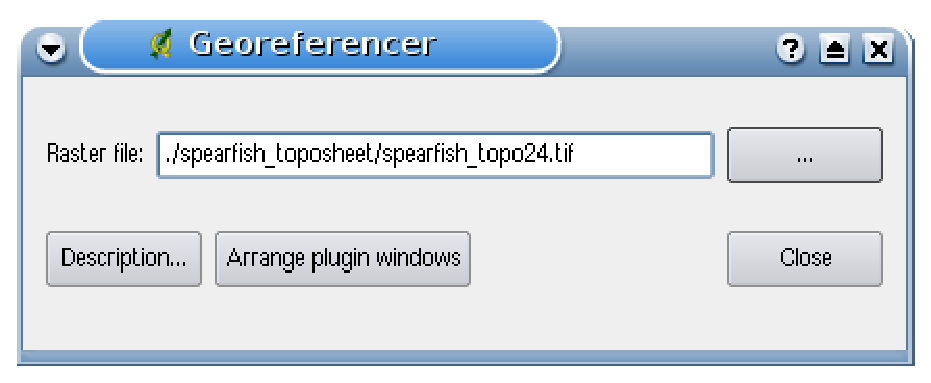
\includegraphics[clip=true, width=12cm]{select_image}
%\end{center}
%\end{figure}

Ora cliccare il pulsante \button{Organizza le finestre di plugin} per aprire l'immagine nel georeferenziatore e organizzarla nella mappa di riferimento della mappa QGIS sulla propria scrivania (Vedere Figura \ref{fig:georefplugin}).

\begin{figure}[ht]
\begin{center}
  \caption{Organizzare le finestre di plugin con la mappa QGIS \nixcaption}\label{fig:georefplugin}\smallskip
  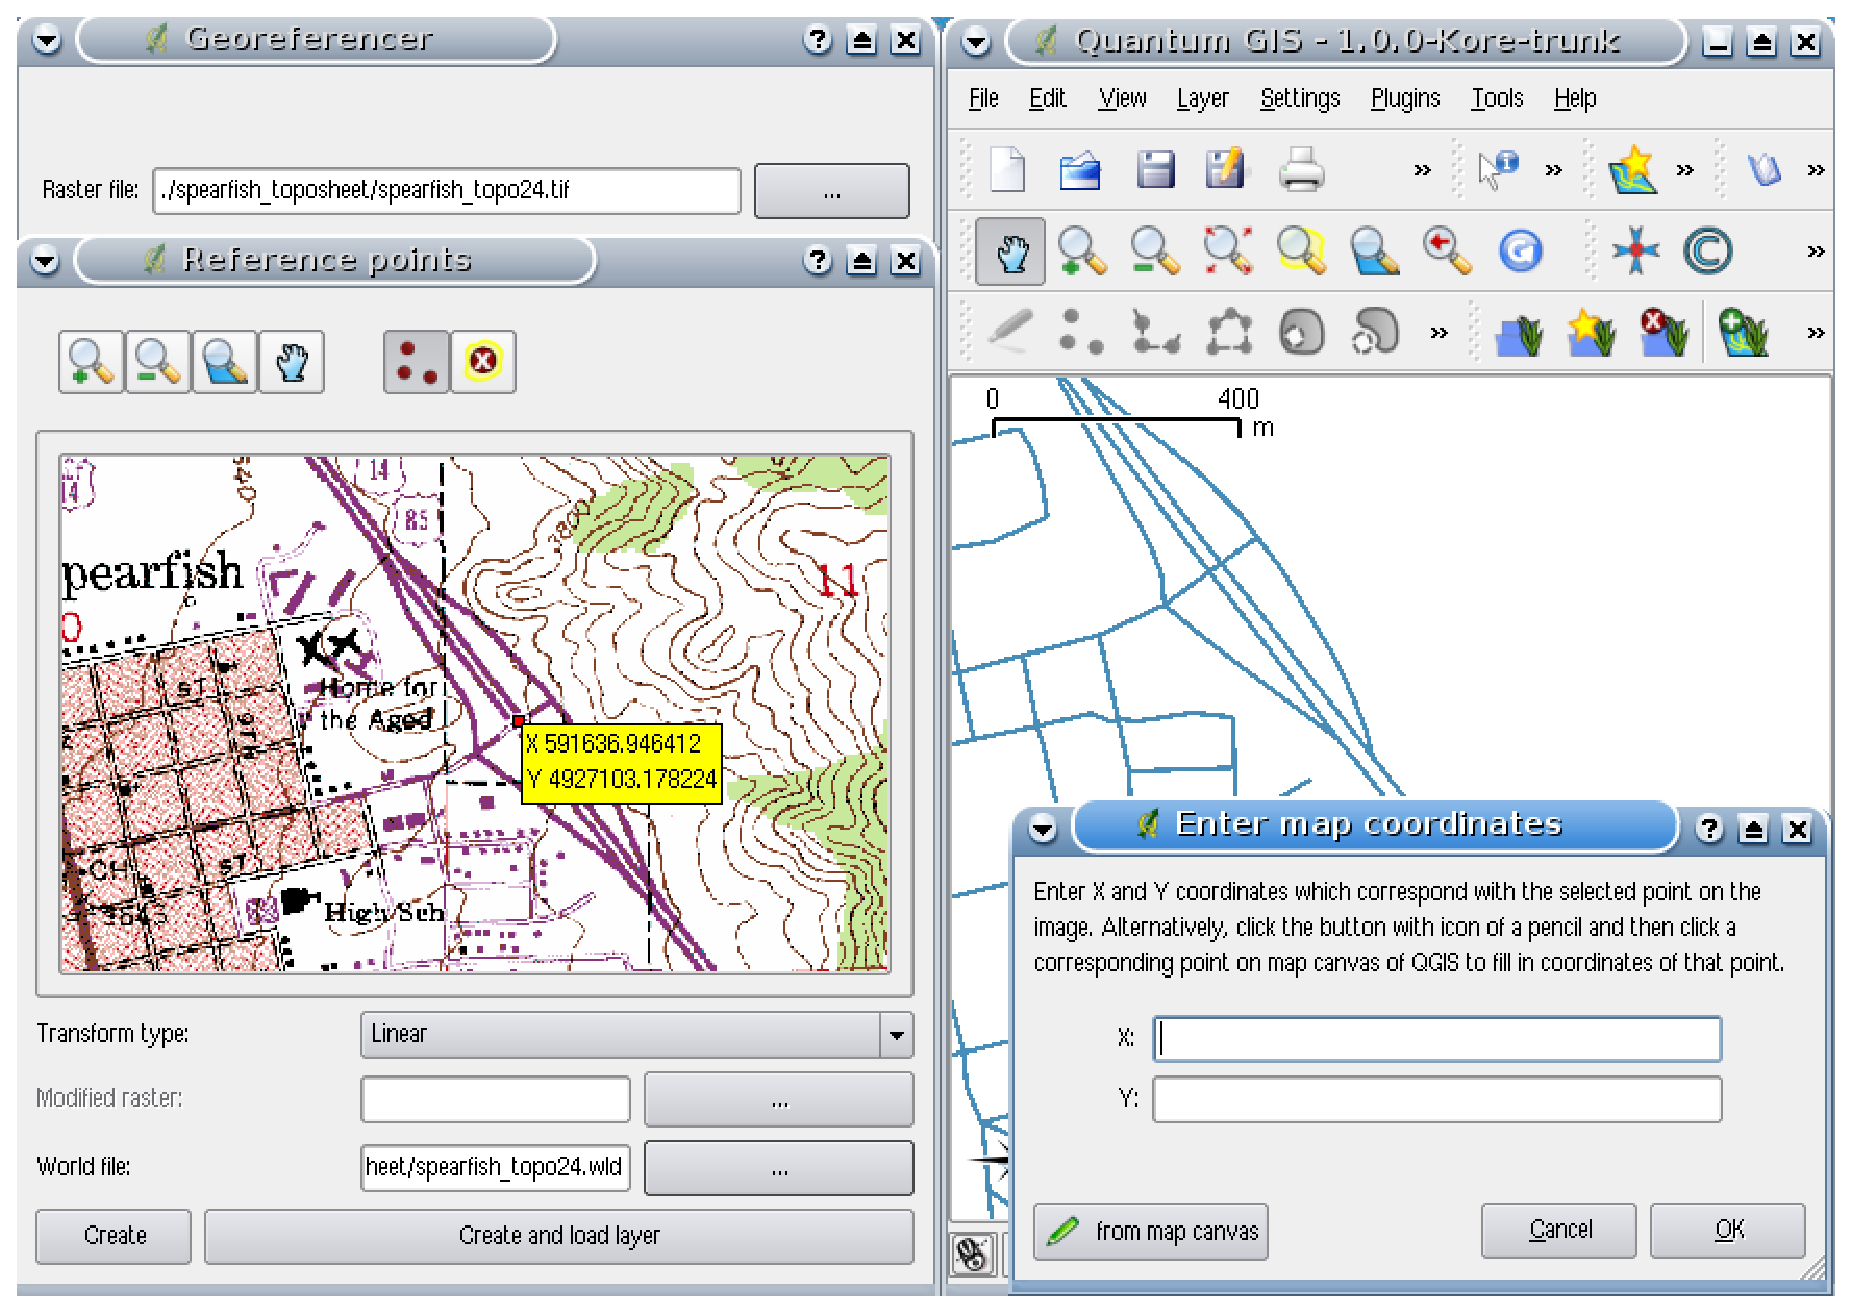
\includegraphics[clip=true,width=\textwidth]{georefplugin}
\end{center}
\end{figure}

Con il pulsante \button{Aggiungi punto} è possibile cominciare ad aggiungere punti sull'immagine raster ed inserire le loro coordinate, il plugin calcolerà i parametri del file di georeferenziazione (Vedere Figura \ref{fig:choose_points}).
Più sono le coordinate che si forniscono, migliore sarà il risultato. Per procedere ci sono due opzioni:

\begin{enumerate}
\item Si può cliccare sul raster inserendo manualmente le coordinate X e Y del punto inserito
\item Si può cliccare sul raster e premere il pulsante \button{da mappa} per aggiungere le coordinate X e Y con l'aiuto di una mappa già georeferenziata già caricata in QGIS.
\end{enumerate}

\begin{figure}[ht]
\begin{center}
  \caption{Aggiungere punti all'immagine raster \nixcaption}\label{fig:choose_points}\smallskip
  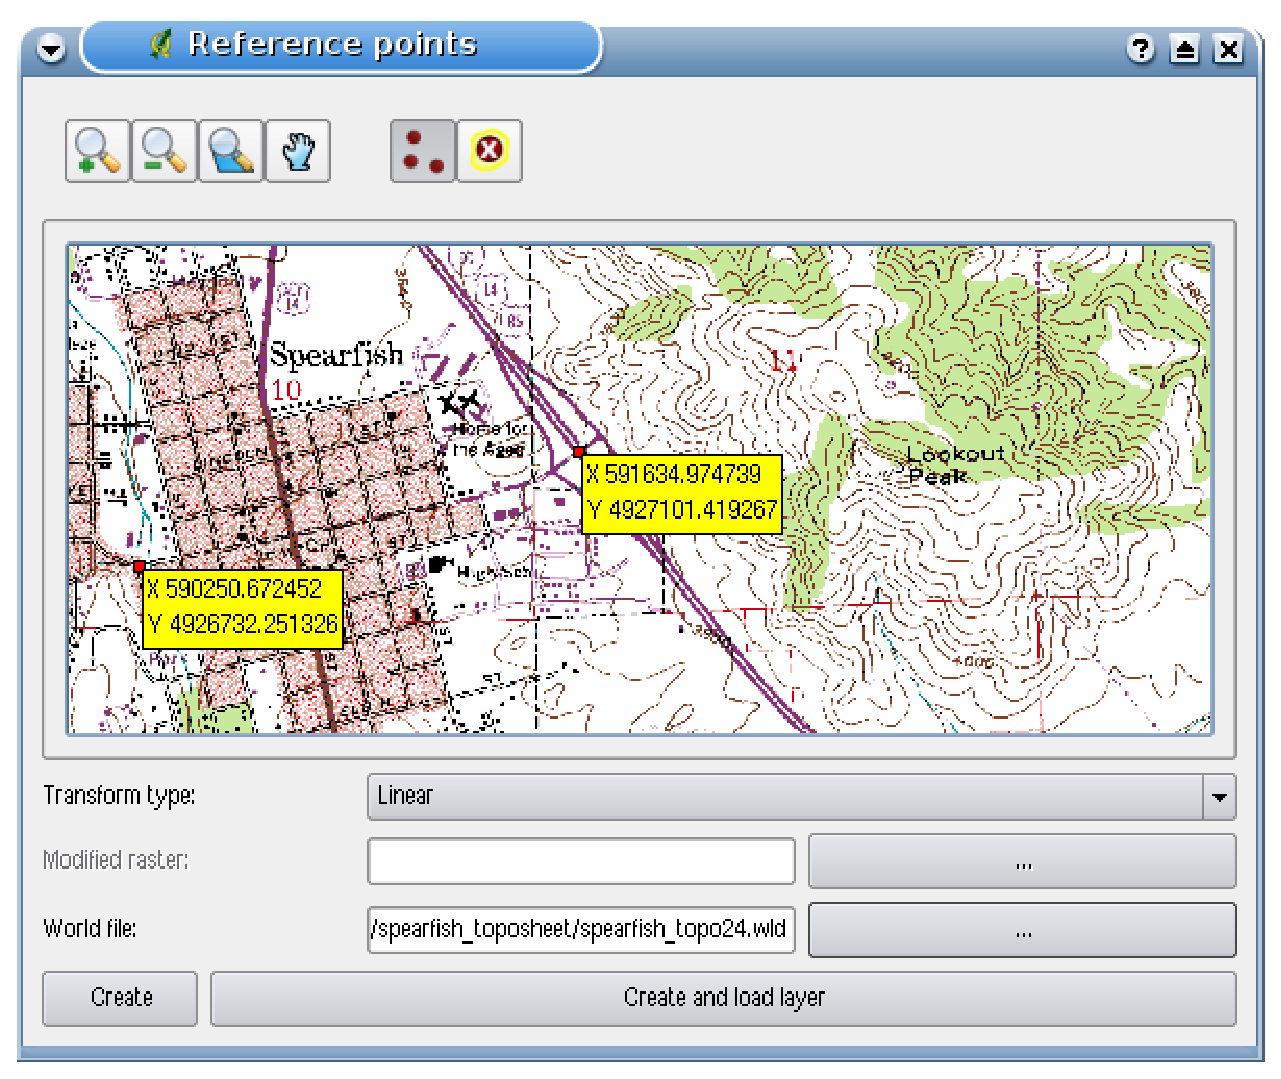
\includegraphics[clip=true,width=0.9\textwidth]{choose_points}
\end{center}
\end{figure}

Per questo esempio useremo la seconda opzione e inseriremo le coordinate per i punti selezionati con l'aiuto della mappa \filename{roads} contenuta nella location \filename{spearfish60} da: \url{http://grass.osgeo.org/sampledata/spearfish\_grass60data-0.3.tar.gz}

Se non si sa come integrare la location \filename{spearfish60} con il plugin GRASS, vedere le informazioni nella Sezione \ref{sec:grass}. Come si può vedere in Figura \ref{fig:choose_points}, il georeferenziatore fornisce tasti di zoom, pan, aggiunta e rimozione di punti dall'immagine.

Dopo aver aggiunti abbastanza punti all'immagine, occorre selezionare il tipo di trasformazione per il processo di georeferenziazione e salvare il risultante file di georeferenziazione insieme con il file Tiff.
Nel nostro esempio scegliamo una
\selectstring{Transform type}{trasformazione lineare} 
anche se una
\selectstring{Transform type}{trasformazione di Helmert}
sarebbe sufficiente.


\begin{Tip}\caption{\textsc{Scegliere il tipo di trasformazione}}
\qgistip{La trasformazione lineare (affine) è una trasformazione di primo ordine e si usa per scalare, traslare e ruotare immagini geometricamente corrette.
Con la trasformazione di Helmert semplicemente si aggiunge l'informazione delle coordinate all'immagine come in un geocoding. Se l'immagine è contorta, è necessario usare software che fornisca trasformazioni polinomiali di secondo o terzo ordine, ad esempio GRASS GIS.}
\end{Tip} 

I punti aggiunti alla mappa saranno salvati nel file \filename{spearfish\_topo24.tif.points} Insieme all'immagine raster. Questo permette di riaprire il plugin Georeferenziatore e aggiungere o rimuovere punti per ottimizzare il risultato. Il file \filename{spearfish\_topo24.tif.points} di quest'esempio mostra i punti:

\begin{verbatim}
mapX    		mapY    		pixelX  pixelY
591630.196867999969982  4927104.309682800434530 591647  4.9271e+06
608453.589164100005291  4924878.995150799863040 608458  4.92487e+06
602554.903929700027220  4915579.220743400044739 602549  4.91556e+06
591511.138448899961077  4915952.302661700174212 591563  4.91593e+06
602649.526155399973504  4919088.353569299913943 602618  4.91907e+06
\end{verbatim} 

Usiamo le 5 coordinate dei punti per georeferenziare l'immagine raster. Per ottenere un risultato corretto, è importante posizionare i punti con regolarità nell'immagine. Infine, si può controllare il risultato, caricare la nuova mappa georeferenziata \filename{spearfish\_topo24.tif} e sovrapporla alla mappa \filename{roads} della location \filename{spearfish60}.

\begin{figure}[ht]
\begin{center}
  \caption{Mappa georeferenziata con la mappa roads della location spearfish60 sovrapposta
  \nixcaption}\label{fig:result_map}\smallskip
  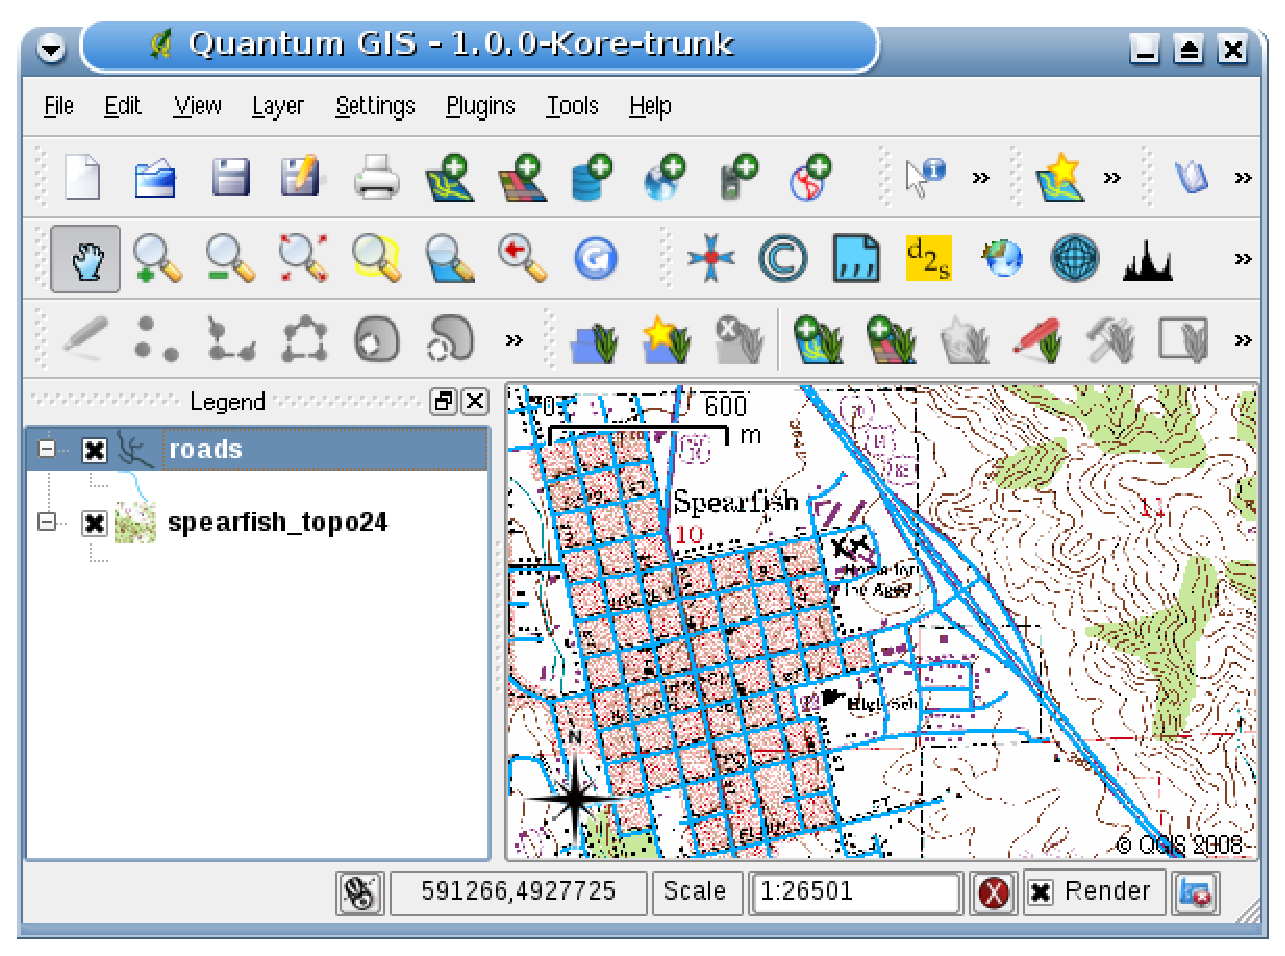
\includegraphics[clip=true,width=\textwidth]{result_map}
\end{center}
\end{figure}
